% Chapter 1
\setstretch{1.8}
\chapter{Algorithms and Flowcharts} % Write in your own chapter title
\label{Chapter4}
\lhead{Chapter 4. \emph{Algorithms and Flowcharts}} % Write in your own chapter title to set the page header

This chapter discusses the process as defined by the IEC standard, and the algorithms and their flowcharts developed to automate the process of motor testing. As described in earlier chapters, the systems were implemented in Simulink and the calling scripts were written in MATLAB.

\section{The Process as defined by IEC-60034-2-1}
Following figure is taken from IEC-60034-2-1:2014 which shows the tests to be performed for separating the losses of an induction motor, smaller than 2 MW.
\begin{figure}[htbp]
	\centering
		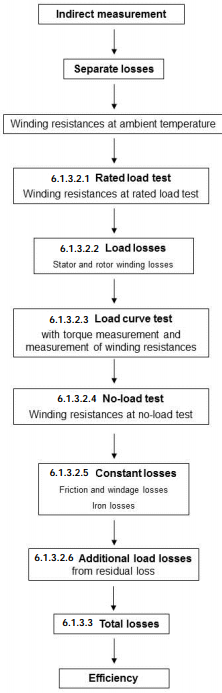
\includegraphics[width = 2.5in]{./Figures/MS/fig41.png}
		\rule{35em}{0.5pt}
	\caption{IEC 60034-2-1 method 2-1-1B, for induction motors}
	\label{fig:IEC 60034-2-1 method 2-1-1B, for induction motors} 
\end{figure}
\newpage

\section{Flowcharts}
\subsection{Rated load test}
The first test in the IEC standard method was the rated load test. In this test, the motor is loaded to its rated power, and is allowed to run till it reaches the thermal equilibrium, and the voltage, current, input power, speed, torque and temperature need to be measured.
Once the test is complete, the stator copper losses are calculated from the data using I\textsuperscript{2}R, and then a temperature correction is applied using temperature correction factor k. The process is illustrated by the following flowchart:
\begin{figure}[htbp]
	\centering
		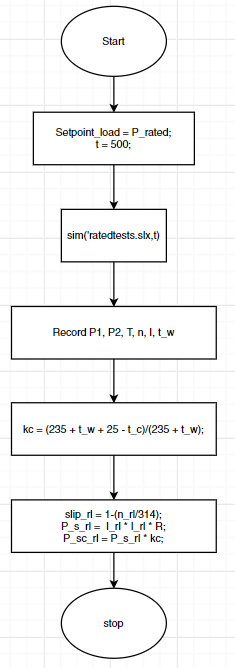
\includegraphics[width = 2.5in]{./Figures/MS/fig42.png}
		\rule{35em}{0.5pt}
	\caption{Rated load test flowchart}
	\label{fig:Rated load test flowchart} 
\end{figure}
\newpage

\subsection{Load Curve test}
The next test in the IEC standard method is the load curve test. In this test, the motor is loaded  to 6 different load points (125\%, 115\%, 100\%, 75\%, 50\%, 25\%), and is allowed to run till it reaches the thermal equilibrium, and the voltage, current, input power, speed, torque and temperature need to be measured.
Once the test is complete, the stator copper losses are calculated from the data using I\textsuperscript{2}R for each load point and then a temperature correction is applied using temperature correction factor k. The process is illustrated by the following flowchart:
\begin{figure}[htbp]
	\centering
		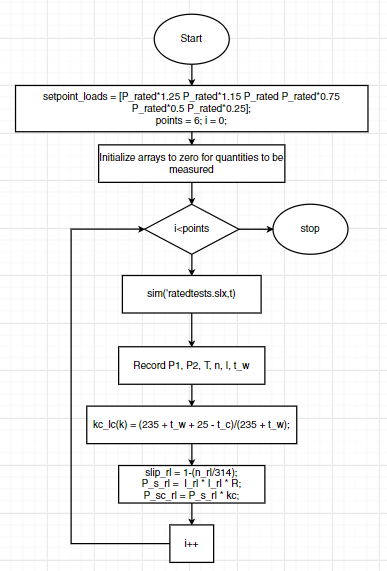
\includegraphics[width = 4.5in]{./Figures/MS/fig43.png}
		\rule{35em}{0.5pt}
	\caption{Load curve test flowchart}
	\label{fig:Load curve test flowchart} 
\end{figure}
\newpage

\subsection{No Load test}
The no-load test consists of two stages. In the first stage, the motor is allowed to run at its rated speed and the input power, voltage and current are measure. The output power is assumed zero in the case as there is no loading torque. In the next stage, the motor is disconnected from the source, and rotated to its rated speed using another motor, and the torque required to run the motor at its rated speed is measured. This torque, multiplied by the motor rated speed, provides us with the friction and windage losses. The iron losses are calculated by subtracting friction and windage losses and no load stator copper losses from the no load input power measured in the first stage. The process is illustrated by the following flowchart:
\begin{figure}[htbp]
	\centering
		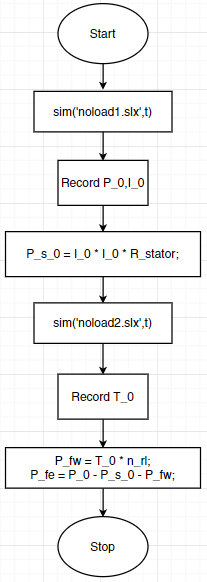
\includegraphics[width = 2.2in]{./Figures/MS/fig44.png}
		\rule{35em}{0.5pt}
	\caption{No load test flowchart}
	\label{fig:No load test flowchart} 
\end{figure}

\newpage
\subsection{Rotor loss and Additional losses}
The rotor copper losses are calculated for each load point by subtracting stator copper loss and iron loss from input power for each step and multiplying it by the slip. After this, the additional load losses can be calculated simply by subtracting all the losses from the input power for each load point. The process is illustrated by the following flowchart:
\begin{figure}[htbp]
	\centering
		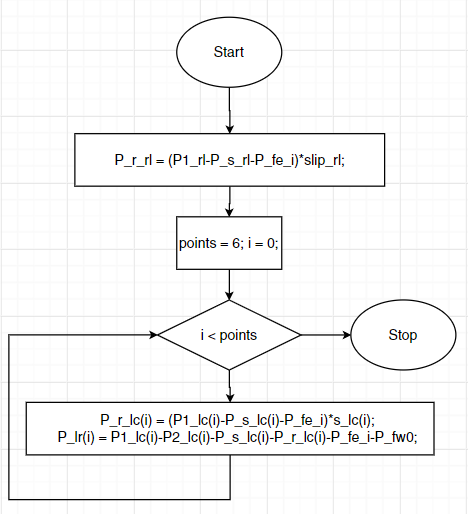
\includegraphics[width = 4.5in]{./Figures/MS/fig45.png}
		\rule{35em}{0.5pt}
	\caption{Rotor loss and PLL calculation flowchart}
	\label{fig:Rotor loss and PLL calculation flowchart} 
\end{figure}

\section{MATLAB scripts}
This section shows the scripts written in matlab to implement the above mentioned flowcharts.
\lstset{language=Matlab,%
    %basicstyle=\color{red},
    breaklines=true,%
    morekeywords={matlab2tikz},
    keywordstyle=\color{blue},%
    morekeywords=[2]{1}, keywordstyle=[2]{\color{black}},
    identifierstyle=\color{black},%
    stringstyle=\color{mylilas},
    commentstyle=\color{mygreen},%
    showstringspaces=false,%without this there will be a symbol in the places where there is a space
    numbers=left,%
    numberstyle={\tiny \color{black}},% size of the numbers
    numbersep=9pt, % this defines how far the numbers are from the text
    emph=[1]{for,end,break},emphstyle=[1]\color{red}, %some words to emphasise
    %emph=[2]{word1,word2}, emphstyle=[2]{style},    
}

\newpage
\section*{Rated load test script}
\lstinputlisting{ratedloadtest.m}

\section*{Load curve test script}
\lstinputlisting{loadcurvetest.m}

\section*{No load test script}
\lstinputlisting{noloadtest.m}

\section*{No load test script(alternate)}
\lstinputlisting{noloadtest.m}

\section*{Rotor loss and PLL calculation script}
\lstinputlisting{rotor_loss_later.m}
